%!TEX root = ../Thesis.tex
\chapter{The Aggregator} % (fold)
\label{cha:aggregator}%\marginnote{The original contribution of this chapter is the functional aggregator reference architecture.}
\newchapter{T}{he concept of aggregators} has become widespread in the smart grid literature. It is clear from the different uses it is given that the concept is still not clearly defined. This chapter contributes to the field of smart grid by making an encompassing definition of what an aggregator is, as well as defining an aggregator lexicon. Furthermore, a functional reference architecture is presented, which establishes the essential functions aggregators must possess for effective service provision. This contribution is important for evaluating the capabilities of aggregators and, by extension, easing the proliferation of aggregators in the power system. Thus, the focus of this chapter is to consolidate the understanding of what an aggregator is in order to harmonize research and discussion around aggregators. Most of the concepts presented here were originally present in as a work-in-progress conference paper\fcite{bondy2015a} which can be found in Appendix~\ref{app:etfa2015}. 

\section{Background}
\newsection{I}{n this work the} concept of aggregation encompasses the creation and management of a portfolio of DERs\footnote{DERs can be referred to flexibility resources, or flexibility assets, when they form part of an aggregation portfolio} which seeks to provide the pooled flexibility in power consumption/production as a service or product to the power system\todo{Should it be power market participants instead of power system?}. This general definition covers most uses of the word in the literature, but there is a large variation in the expected functionality of these aggregators. This can be seen by the wide variety of aggregator designs in the literature\footnote{See \eg\cite{kok2005powermatcher,han2010development,sortomme2011optimal,costanzo2013coordination}.}. The main reason for this has been the fact that aggregators have been designed for specific kinds of units, for specific market rules and for specific services. An aggregator taxonomy is helpful for reaching a common understanding of what an aggregator is (and is not) expected to do, and how it is anticipated to perform.

In some works\fcite{fenix2009} a distinction between aggregators is made in terms of which kind of task they perform. If they provide ancillary services they are catalogued as Technical \Glspl{vpp} and if they trade energy in the day-ahead energy market they are catalogued as Commercial VPPs. But recent work\fcite{niesse2014conjoint} proposes a \emph{Dynamic VPP}, which is an aggregator that is designed to participate both in day-ahead markets and ancillary service markets. This type of advanced design could become commonplace in future, making the \emph{Commercial} vs. \emph{Technical VPP} classification obsolete.

Other works classify\fcite{kosek2013overview} aggregators based upon their control paradigm into autonomous, direct, indirect and transactional control. While this classification is more robust towards future aggregator designs, it falls short on one main issue: \emph{where is the intelligence located?}. In other words, the responsibility\footnote{The concept of responsibility is central to the operation of the power system, since it determines which market player is to pay for system imbalances.} and location of decision making is not taken into consideration in this classification. The responsibility and location of the decision making impacts the internal payment settlement of the aggregator, the scalability of the solution, the robustness towards communication faults and the time response capabilities, therefore it must be taken into account. In order to do this, a new taxonomy has been proposed\fcite{han2016review}, which identifies six classes of aggregator architectures ranging from the fully centralized decision making, to the fully autonomous\footnote{The control paradigm classification can be considered a further sub-classification within this taxonomy.}. This taxonomy is currently the one that falls the best in line with the ideas presented in this work\todo{should I go into details here with respect to the control mechanisms?}.

\section{Clarifying the Aggregator Concept}
\newsection{R}{esponsibility is a central} concept within power systems. While it is technically possible to provide DR-ancillary services without an aggregator, it is impractical for each DER owner to enter into a contractual agreement for rendering services to the system operators\footnote{The term System Operators is used here to refer to both Transmission System Operators and Distribution System Operators.}. In this sense, the aggregator becomes a legal entity that absorbs the legally binding responsibility of its customers and ensures that the aggregated portfolio follows an aggregated operation schedule. At the same time, the aggregator has an ICT infrastructure, which encompasses both the communication and decision making of the aggregator. It uses this infrastructure to coordinate the DERs/flexibility assets' behavior to match a service need of a higher volume than what an individual unit would be able to cover. Also, the aggregator entity will typically not own the flexibility assets it controls. This multi-domain approach to defining aggregators can be seen in Figure~\ref{fig:MAINdomains}\footnote{This figure is an adaptation of the one presented in \cite{bondy2015a} which can be found in Appendix~\ref{app:etfa2015}}.

\begin{figure}[htbp!]
\centering
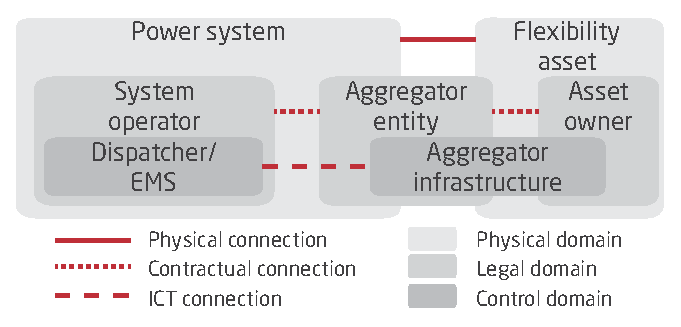
\includegraphics[width=1.0\textwidth]{domains3.eps}
\caption{The aggregator concept across domains. The aggregator is present in the physical domain with the ICT system, the legal domain through its service contracts, and the control domain through its decision making logic regarding the behavior of the flexibility assets.}
\label{fig:MAINdomains}
%\vspace*{-5mm}
\end{figure}

These concepts lead to the following definitions:
\begin{description}
	\item[Aggregator role:] The role in the power system of performing aggregation with the purpose of selling the flexibility in consumption or production. The sale of flexibility can be a service to System Operators or it can be traded in day ahead markets. The aggregator role can be assigned to a new player in the markets, or it can be assigned to an existing player, \eg a Balance Responsible Party or a utility.\todo{Include USEF definition}
	\item[Aggregator entity:] The legal entity of the aggregator, which enters into contractual agreements with the other market players and flexibility asset owners. This entity is legally responsible for living up to the contractual agreements.
	\item[Aggregator infrastructure:] The communication and control infrastructure, both in terms of software and hardware, that the aggregator owns and operates in order to control the flexibility assets. \todo{Discuss with Kai and Oliver, I think I'm messing up some terms here}
	\item[Aggregator architecture:] The shape of the aggregator infrastructure. This encompasses not only the control strategy, but a series of essential functions which will be described in Section~\ref{sec:MAINaggrefarch}.
	\item[Aggregator:] The term used to refer to a market player that has an aggregator role, entity and infrastructure.
\end{description}

Aggregators provide two kinds of services\footnote{The terminology used in Appendices~\ref{app:etfa2015} and \ref{app:isgt2014} varies slightly from the one presented here. The terms used in this section are considered definitive.\bondy{I'm not sure the wording is right here}}:
\begin{description}
	\item[Flexibility services] which are provided to System Operators and BRPs. These will take the form of ancillary services for the TSO, distribution system services for the DSO and portfolio balancing services for the BRP\footnote{The mentioned types of services will be expanded upon in Chapter~\ref{cha:services}.}.
	\item[Asset management services] provided to the owners of the units, which consists of managing the flexibility asset for the owner, so that it can participate in the flexibility service provision, while still respecting the primary use/comfort settings of the asset owner.
\end{description}
This is shown in Figure~\ref{fig:market_futureMAIN}, where the aggregator is selling services to the System Operators through the Consumption BRP. This is a market setup which was concluded upon in the iPower project. Other market setups allow for the aggregator to participate directly in the market, as long as they coordinate with their corresponding Consumption BRP, such that the aggregator avoids provoking imbalances to the Consumption BRP.
\begin{figure}[htbp!]
\centering
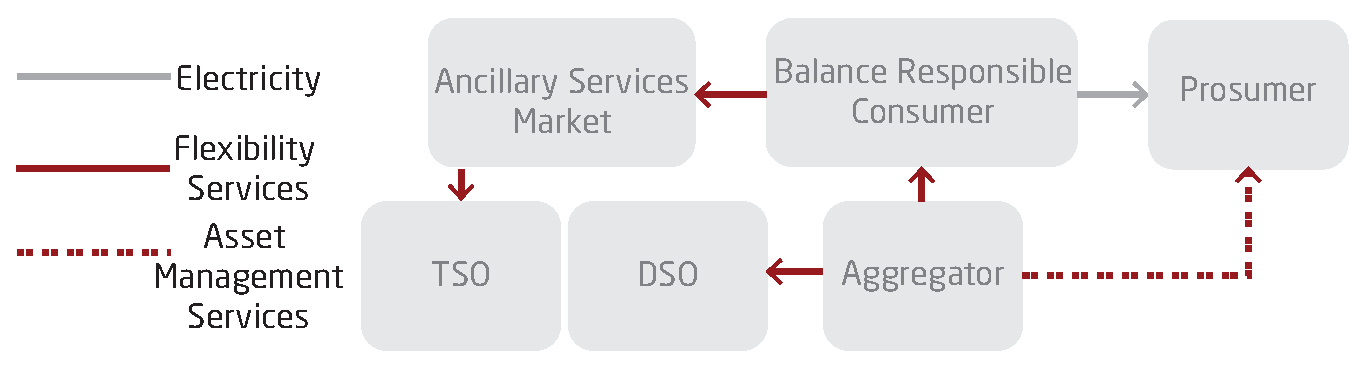
\includegraphics[width=1.0\textwidth]{market_futureMAIN.eps}
\caption{The aggregator as a service provider. This figure is a modified version of Figures~\ref{fig:marketfuture} and \ref{fig:SEGANmarket}.}
\label{fig:market_futureMAIN}
%\vspace*{-5mm}
\end{figure}

Another concept that needs to be defined is the one of \emph{flexibility}. The word has been used loosely as the amount of power consumption/production a unit is able to deviate from a plan, within the constraints set by the primary function of the unit, \eg transportation in the case of an EV. To expand upon this concept of flexibility, two kinds of flexibility are considered: \emph{deferred} and \emph{non-deferred} flexibility. When flexibility is provided as a \emph{non-deferred} flexibility,  it means that the consumption/generation is reduced/increased without the need to recuperate/shed the energy provided in the service. Correspondingly, \emph{deferred} flexibility is where the units providing the service need to return to a nominal state by recuperating or shedding energy. In demand response, the latter is the most common kind of flexibility used. Consequently, flexibility has two dimensions:
\begin{itemize}
	\item A power (or energy) component, at a given volume and granularity, which the aggregator can offer, and
	\item A time component, which affects:
		\begin{itemize}
			\item the time horizon over which the change in consumption/production can be sustained, and/or
			\item the time granularity of the offered flexibility\footnote{The time and power granularities are important if the service is provided by units whose main process has time constraints, \eg minimum on-time for compressors, and power constraint, \eg only on-off capabilities of the full power rating.}.
		\end{itemize}
\end{itemize}

A flexibility taxonomy was proposed by \emph{Petersen et al.}\fcite{petersen2013taxonomy} where flexibility is catalogued as \emph{buckets}, \emph{batteries} and \emph{bakeries}, and in \emph{Hansen et al.}\fcite{hansen2014demand} it is shown how this taxonomy can be applied to a comprehensive set of DR schemes. While this taxonomy covers both the power and time components in terms of magnitude, the granularity is only addressed in the case of the time component. This means that the taxonomy does not take the power granularity of the flexibility into account. Under the current assumption, \ie that flexibility services will be provided by a large amount of small-size units, this limitation of the taxonomy is irrelevant. However, if the volume requirements for services are reduced in the future, thus enabling aggregators with small portfolios, it might be relevant to further expand the flexibility taxonomy. This could, for example, be done by splitting the categories into \emph{continuous} and \emph{discrete} buckets, batteries and bakeries.

Finally, one of the central points of this work is that aggregators are essentially different from traditional generators. Aggregators differ from traditional generators in the sense that\footnote{The differences pointed out here are further expanded upon in Section~\ref{subsec:backgroundvalidation}.}:
\begin{enumerate}
	\item they are distributed systems where each unit has its own response properties, therefore the overall response behaves very differently than that of traditional generators;\label{point:aggblackbox}
	\item they have no single point of measurement, which means the traditional measuring requirements can not be met;
	\item reliability concepts must be adapted to their distributed nature, both in terms of communication reliability and service reliability;
	\item aggregator architectures will vary widely, and each architecture will be sensitive to different operation scenarios;
	\item while traditional generators follow operational schedules, \ie they have a baseline, aggregators are not required to follow schedules in the same way;
	\item the primary use of the flexibility assets is to satisfy its owner's need, not to trade power consumption/production in the electricity markets, and it may be that the asset is part of a larger process.
\end{enumerate}

%While the dynamics of fossil-fueled power plants are well understood and can be modelled based upon physical equations, aggregators can only be analyzed as black boxes.
\section{Advantages and Limitations of Aggregators}
\newsection{A}{s stated in the} previous section, the aggregator is a cross-domain entity. Most of the literature on aggregators and demand response focuses on the advances in the control domain which bring \emph{operating}, \emph{planning} and \emph{economic} advantages to the power system\fcite{oconnell2014benefits}. In this work the focus is on the \emph{operating} advantages brought by aggregators, which can divided into three categories: \emph{scalability}, \emph{reliability} and \emph{responsiveness}.

In the control domain,\marginnote{The concepts described in this section are focused on aggregators as service providers, but the same concepts can be applied for aggregators trading in the day-ahead or intra-day markets.} the advantages of contracting an aggregator instead of a large amount of individual small sized units are similar to those of the legal domain. That is, the aggregator in its essence can be regarded as a solution for \emph{scalability} of the smart control of flexible consumption or production. It would be possible for a System Operator to directly engage all customers in order to buy services, but the coordination of such large quantities is impractical for the System Operators. Thus, the System Operators can request fewer services with large volume, and the aggregator will then supply this service with its portfolio of units.

Aggregators providing services through demand response can be more reliable that their traditional counterpart\fcite{kirby2007load,callaway2011a}. This is due to the fact that a fault in one large generator will have a much higher impact than faults in several smaller-sized units. This makes for an argument for aggregators improving the \emph{reliability} of power system.

Lastly, most DERs have very fast response times, which means that compared to traditional coal-fueled power plants, aggregators are able to provide very fast services. This implies that frequency excursions can be stopped faster and at a higher frequency nadir\fcite{vrettos2015integrating}. This leads to system operators requiring smaller reserves for maintaining  the system security\fcite{makarov2008assessing}.

The main technical limitation on aggregators is that most DERs have as a main objective to satisfy the needs of it's owner, \eg transportation in the case of EVs or heating in the case of HPs. Thus, the aggregator is constrained in its flexibility by the primary function of the DERs. Similarly, selling flexibility through aggregators is optional, so an aggregator must make a compelling business case for the DER owner to participate in the service markets.

Another technical limitation is directly related to the kind of flexibility the aggregator provides. In most cases the aggregator will use \emph{deferred} flexibility, where the units need to recuperate after the service delivery. If all units in the portfolio recuperate at the same time, the consumption spike that ensues may be a larger problem than the one the aggregator was contracted to solve. This is also known as the kick-back effect\bondy{ask Xue for references}. The problem of saturation can also be associated with this. DERs are usually only able to deliver services on short time horizons (compared to traditional generators) due to the limit size of the units. Once a minimum or maximum state has been reached, the flexibility of the unit disappears. This concept can be represented as a set of saturation curves\fcite{thavlov2015thesis}, where asking for large volumes of power means the units can only deliver for short time periods and vice versa.

A non-technical limitation comes from market regulations. Market rules and ancillary service requirements are defined based on the capabilities of traditional generators. This means that aggregators are expected to behave as traditional generators, when they in essence are something completely different. This means that rules and requirements need to be changed if DER capabilities are to be fully exploited\footnote{This topic is addressed in depth in Chapter~\ref{cha:services}.}.

\section{The Functional Aggregator Reference Architecture}\label{sec:MAINaggrefarch}
\newsection{U}{ntil now, the discussion} on the aggregator has been focused on its role in the power system. In order to further the understanding of what an aggregator is, its functionality must be analyzed. One of the main contributions of the presented research is a \emph{Functional Reference Architecture for Aggregators}. The objective of creating a reference architecture is to address the issue of benchmarking and validation/certification of aggregators\footnote{This topic will be discussed in depth in Chapter~\ref{cha:validation}.}. The traditional approach to certification of generators can not be applied to aggregators, and therefore new methods must be designed. Part of this method is to verify that an aggregator possesses the essential functionality for effective service provision. This essential functionality is defined in the proposed reference architecture.

In order to formulate the aggregator reference architecture, a set of existing commercial and academic aggregators\footnote[][-2em]{The analyzed aggregators were: Open Energi\cite{openenergi}, PowerHub by DONG Energy\cite{powerhub}, the Heterogenous Aggregator by Aalborg University\cite{rahnama2014evaluation} and the D-EMPC\cite{costanzo2013coordination}.}  were decomposed into their basic functionality. The resulting functions are\footnote{For detailed explanations of each function see Section~\ref{sec:funcdec}.}:

\begin{enumerate}[label=\Alph*]
		% external interface
	\item Service Interface: The function that translates information from the legal domain to the control domain\footnote{See Figure~\ref{fig:MAINdomains}.}
		% Monitoring & Supervision modules
	\item Performance Monitoring: The function that evaluates and verifies the behavior of the client unit.
	\item Supervision and Resource Handling: The function that determines the availability and composition of the resource portfolio based upon the performance of the units.
	\item Operator Interface: The function that supports operator decision making.
		% Control related
	\item Control: The function that generates the appropriate control domain signals to manipulate the portfolio behavior.
	\item Flexibility Monitoring: The function that assesses the amount of flexible consumption/production available in the portfolio.
		% Communication
	\item Aggregator-internal Communication: The function that covers the internal communication within the distributed elements of the aggregator.
	\item Client Management: The function that determines the availability of the flexibility assets depending on their communication status.
	\item External Information Services: The function that pulls the necessary external data for the functioning of the aggregator, \eg weather and price forecasts.
	\item Asset Interface: The function that translates between the control domain signals and the specific protocols used by the flexibility asset.
		% The odd one out
	\item Internal-information exchange: The function that enables the exchange of data and other information between the relevant functions of the aggregator.
\end{enumerate}

Conceptually, each function has a specific purpose and task, but in the actual software implementation of the aggregator, one or more of these functions may be executed in the same module. The functions can be classified in two different ways: a task based classification and a data-handling based classification. The task based classification divides the functions according to the kind of task the function executes:
\begin{description}
	\item[External interface:] The functions that provide information exchange with entities outside the aggregator infrastructure.
		\begin{itemize}
			\item Service Interface: Outputs a serviced model that sets the objective of the aggregator.
			\item Asset Interface\footnote{The asset interface may also be considered part of the communication related functions, since it provides the communication translation between the flexibility asset and the rest of the aggregator infrastructure.}: Outputs the DER/flexibility asset data to the rest of the aggregator.
		\end{itemize}
	\item[Monitoring \& Supervision:] The functions that parse information related to the unit portfolio.
		\begin{itemize}
			\item Performance Monitoring: Outputs the performance of the individual and aggregated flexibility assets. Can be used for internal purposes and/or service settlement purposes.
			\item Supervision and Resource Handling: Outputs the portfolio that is available for control, based upon the performance/compliance of the units.
			\item Operator Interface: Outputs manual decisions with respect to the portfolio and control.
		\end{itemize}
	\item[Control related functions:] The functions that involve the automated decision making with regards to the unit behavior manipulation.
		\begin{itemize}
			\item Control: Outputs control domain signals, \eg activation or reference signals to the flexibility assets. This is highly dependent on the specific control architecture that the aggregator implements.
			\item Flexibility Monitoring: Outputs the state of the DERs/flexibility assets in terms of the flexibility available for control.
		\end{itemize}
	\item[Communication:] The functions that relate to the internal communication of the aggregator.
		\begin{itemize}
			\item Aggregator-internal Communication: Passes information
			\item Client Management: Outputs the portfolio of connected and responsive units.
			\item External Information Services\footnote{Since the external information services only pull information from outside of the aggregator, and no information exchange is carried out, this function is not considered part of the external interface functions.}: Outputs the required external data.
		\end{itemize}
	\item[Knowlegde exchange:] This category only covers the Internal-information Exchange. It enables the information exchange between all parts of the aggregator. It can take any form, from a simple bus to highly developed data storage system, and has no specific output by itself.
\end{description}
This classification is represented in Figure~\ref{fig:MAINrefarch} through the symbols marked on each function block.

The data-handling based classification is done by grouping the functions based on how data/information is handled in the function. This classification is reflected in Figure~\ref{fig:MAINrefarch} through the color code. The function classes are the following:
\begin{description}
	\item[Enabler functions:] Those functions that only pass the data/information on to other functions.
	\item[Information interpreters:] Those functions that convert data into information.
	\item[Decision making functions:] Those functions that use the information to make decisions.
\end{description}

The functions defined here abstract from any kind of aggregator architecture implementation, and provide the building blocks for the functional reference architecture shown in Figure~\ref{fig:MAINrefarch}\footnote{This diagram is a correction of the one presented in Appendix~\ref{app:etfa2015}.}. Arrows representing data flow were avoided in the design, since they presuppose a specific aggregator architecture. Given that the functional reference architecture must be as encompassing as possible, it should not reflect any specific aggregator architecture implementation, \eg centralized decision making vs. distributed decision making architecture. 
\begin{figure}[htb]
\centering
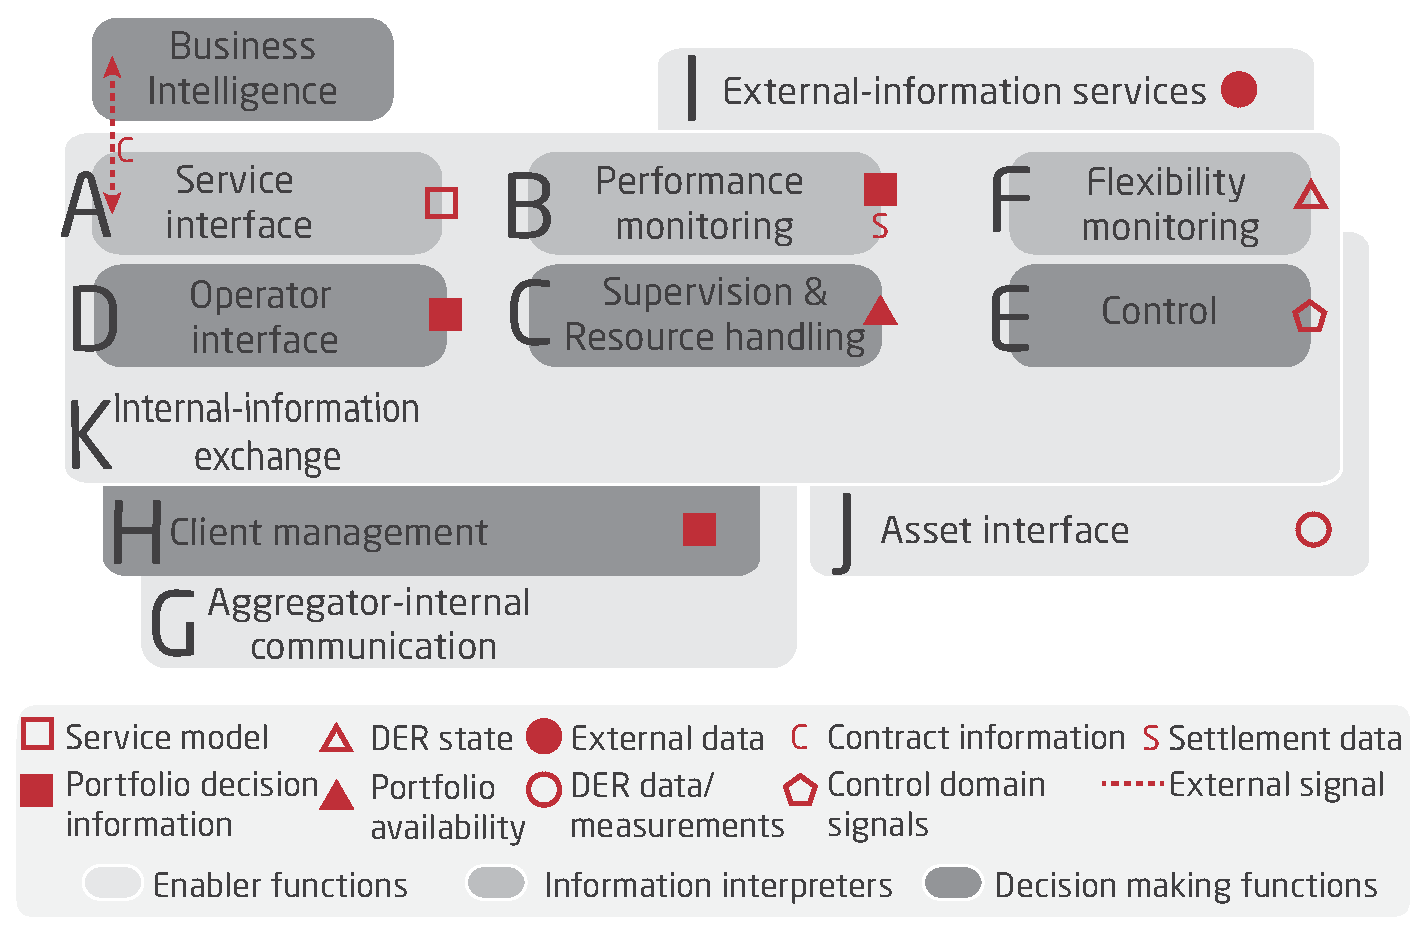
\includegraphics[width=1.0\textwidth]{diag_simple3.eps}
\caption{A visual representation of the proposed reference architecture. The symbols represent data types that are outputs to the functions, and the color represents the data-handling categorization of the functions.}
\label{fig:MAINrefarch}
\end{figure}

\section{Aggregator Maturity Assessment}
The concept of aggregator validation is discussed in depth Chapter~\ref{cha:validation},

The presented functional reference architecture

\section{Conclusions Regarding Aggregators}
\newsection{T}{he concept of aggregators} is widespread in the smart grid literature, but the interpretations of what an aggregator is varies widely. One of the contributions presented in this chapter is to provide a common lexicon and reference architecture for aggregators so that discussion on the topic can be harmonized. This will hopefully lead to faster advances in the field. Also, the functional reference architecture is to be used in aggregator validation and certification\footnote{The concept of aggregator validation and certification is discussed in depth in Section~\ref{sec:aggpreq}, where it is also discussed how this functional reference architecture can be useful.}. A secondary use for the reference architecture is to serve as a guide for future designs of aggregators.

A current shortcoming of this work is that the presented functional reference architecture for aggregators is part of a work-in-progress paper and as such, needs to be refined and extended. Future work will include the design of key performance indices (KPIs) assigned to each function, such that the scores can be used for benchmarking. 

The next chapter will present a deeper analysis and justification for aggregator validation and certification.
% chapter The Aggregator (end)
